\subsection{Testing testing...}
This is where the testing results go

some numbers for now: Transfers running since March, some 2.6 million transfers, 87\% success
rate, over 2 PB of data so far. This is approximately 7\% of the rate CMS achieves globally.

% Points to make:
% testbed running on and off for over a year, transferring files between pairs of sites in both directions, driven by LifeCycle agent
% used initially for debugging and functionality checks
% also used for specific testing: comparing IPv4 with IPv6 performance, testing with different file-sizes
% since March 2013, running continuously, with up to 11 sites. 1 GB file each-way, continuously. As number of nodes increased, add a delay between successive transfers to avoid overloading sites
% discuss results of figure full-mesh
% 2.6 M transfers, 87\% success, over 2 PB transferred, which is ~ 7\% of global CMS rate

% PhEDEx transfers. using private PhEDEx instance and nodes. DPM and FTS3. Transfers throttled to avoid overload. PhEDEx now shown to run with IPv6 endpoints.
% Simon/Duncan to describe this bit better

% To create this graphic:
% 1) save your image as a 1024x1024 png/gif/bmp
% 2) convert to pdf (install ImageMagick, then 'convert FileIn.png FileOut.pdf')
% N.B. if the input and output files have the same base name, LaTeX will prefer to take the png over the pdf,
% which is probably not what you want. Make sure the files have different names!
\begin{figure}[htp]
\centering
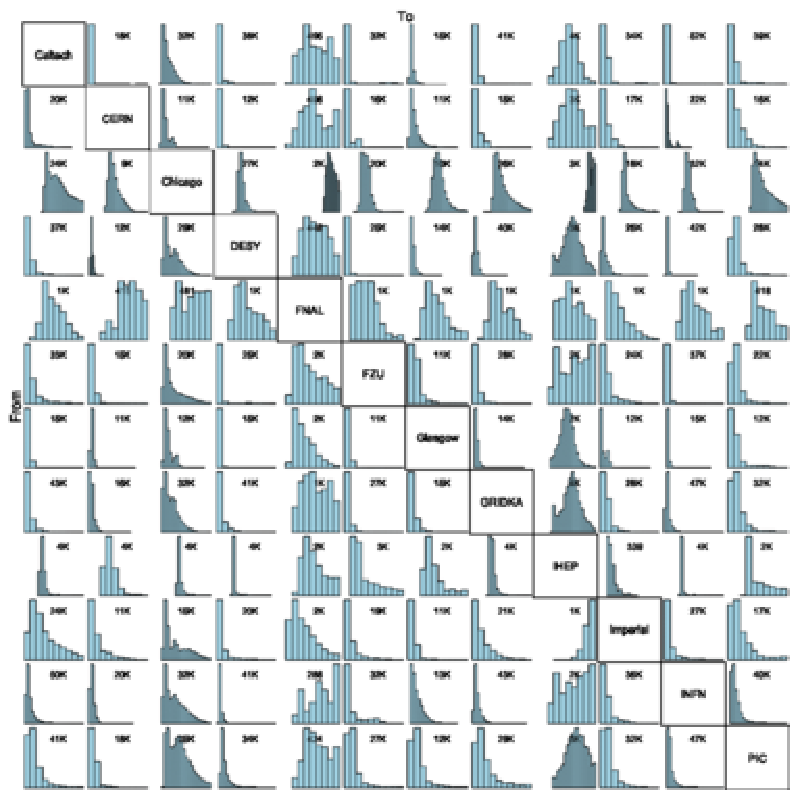
\includegraphics{full-mesh}
\caption{Transfer performance for the IPv6 testbed continuous transfers. A 1 GB file is transferred between each pair of sites, then deleted, then transferred again, continuously. The plots show the distribution of transfer duration times per site pair. The source site is named in the row, the destination site is named in the column. So the top-right plot shows transfers from Caltech to PIC, the bottom-left shows transfers fromPIC to Caltech. The x-axis is in seconds, from 0 to 500 for each plot. The number inset in each plot shows the approximate number of transfers between that site pair in that direction.}\label{fig:full-mesh}
\end{figure}

\begin{figure}[htp]
\centering
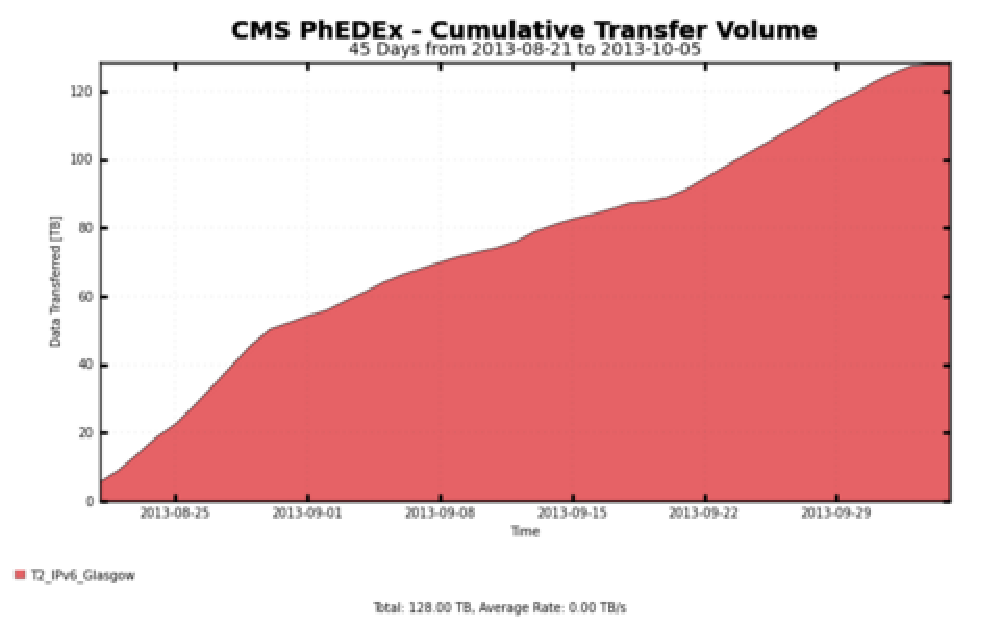
\includegraphics{phedex-transfer-volume}
\caption{Cumulative data-transfer between Imperial College and Glasgow using PhEDEx on the IPv6 testbed.}\label{fig:phedex-transfer-volume}
\end{figure}

